% cpu/cpu.tex
% mainfile: ../perfbook.tex
% SPDX-License-Identifier: CC-BY-SA-3.0

\QuickQuizChapter{chp:Hardware and its Habits}{Hardware and its Habits}{qqzcpu}
%
\Epigraph{Premature abstraction is the root of all evil.}
	 {\emph{A cast of thousands}}

Most people intuitively understand that passing messages between systems
is more expensive than performing simple calculations within the confines
of a single system.
But it is also the case that communicating among threads within the
confines of a single shared-memory system can also be quite expensive.
This chapter therefore looks at the cost of synchronization and communication
within a shared-memory system.
These few pages can do no more than scratch the surface of shared-memory
parallel hardware design; readers desiring more detail would do well
to start with a recent edition of \pplsur{John L.}{Hennessy} and
\pplsur{David A.}{Patterson}'s classic
text~\cite{Hennessy2017,Hennessy95a}.

\QuickQuiz{
	Why should parallel programmers bother learning low-level
	properties of the hardware?
	Wouldn't it be easier, better, and more elegant to remain at
	a higher level of abstraction?
}\QuickQuizAnswer{
	It might well be easier to ignore the detailed properties of
	the hardware, but in most cases it would be quite foolish
	to do so.
	If you accept that the only purpose of parallelism is to
	increase performance, and if you further accept that
	performance depends on detailed properties of the hardware,
	then it logically follows that parallel programmers are going
	to need to know at least a few hardware properties.

	This is the case in most engineering disciplines.
	Would \emph{you} want to use a bridge designed by an
	engineer who did not understand the properties of
	the concrete and steel making up that bridge?
	If not, why would you expect a parallel programmer to be
	able to develop competent parallel software without at least
	\emph{some} understanding of the underlying hardware?
}\QuickQuizEnd

% cpu/overview.tex

\section{Overview}
\label{sec:cpu:Overview}

Careless reading of computer-system specification sheets might lead one
to believe that CPU performance is a footrace on a clear track, as
illustrated in Figure~\ref{fig:cpu:CPU Performance at its Best},
where the race always goes to the swiftest.

\begin{figure}[htb]
\centering
\resizebox{3in}{!}{\includegraphics{cartoons/r-2014-CPU-track-meet}}
\caption{CPU Performance at its Best}
\ContributedBy{Figure}{fig:cpu:CPU Performance at its Best}{Melissa Broussard}
\end{figure}

Although there are a few CPU-bound benchmarks that approach the ideal
shown in Figure~\ref{fig:cpu:CPU Performance at its Best},
the typical program more closely resembles an obstacle course than
a race track.
This is because the internal architecture of CPUs has changed dramatically
over the past few decades, courtesy of Moore's Law.
These changes are described in the following sections.

\subsection{Pipelined CPUs}
\label{sec:cpu:Pipelined CPUs}

\begin{figure}[tb]
\centering
\resizebox{3in}{!}{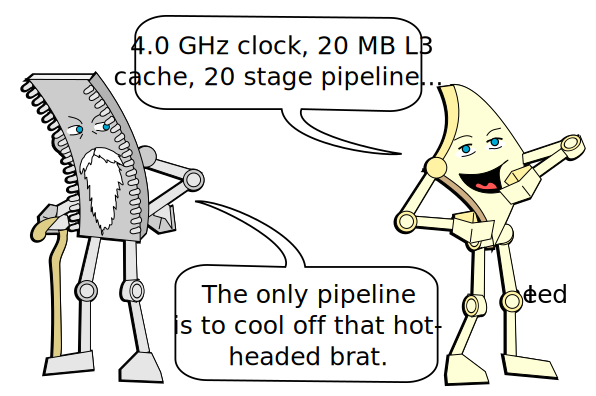
\includegraphics{cartoons/r-2014-Old-man-and-Brat}}
\caption{CPUs Old and New}
\ContributedBy{Figure}{fig:cpu:CPUs Old and New}{Melissa Broussard}
\end{figure}

In the early 1980s, the typical microprocessor fetched an instruction,
decoded it, and executed it, typically taking \emph{at least} three
clock cycles to complete one instruction before proceeding to the next.
In contrast, the CPU of the late 1990s and early 2000s will be executing
many instructions simultaneously, using a deep ``pipeline'' to control
the flow of instructions internally to the CPU.
These modern hardware features can greatly improve performance, as
illustrated by Figure~\ref{fig:cpu:CPUs Old and New}.

Achieving full performance with a CPU having a long pipeline requires
highly predictable control flow through the program.
Suitable control flow can be provided by a program that executes primarily
in tight loops, for example, arithmetic on large matrices or vectors.
The CPU can then correctly predict that the branch at the end of the loop
will be taken in almost all cases,
allowing the pipeline to be kept full and the CPU to execute at full speed.

\begin{figure}[tb]
\centering
\resizebox{3in}{!}{\includegraphics{cartoons/r-2014-branch-error}}
\caption{CPU Meets a Pipeline Flush}
\ContributedBy{Figure}{fig:cpu:CPU Meets a Pipeline Flush}{Melissa Broussard}
\end{figure}

However, branch prediction is not always so easy.
For example, consider a program with many loops, each of which iterates
a small but random number of times.
For another example, consider
an object-oriented program with many virtual objects that
can reference many different real objects, all with different implementations
for frequently invoked member functions.
In these cases, it is difficult or even
impossible for the CPU to predict where the next branch might lead.
Then either the CPU must stall waiting for execution to proceed far
enough to be certain where that branch leads, or it must guess.
Although guessing works extremely well for programs with predictable
control flow, for unpredictable branches (such as those in binary search)
the guesses will frequently be wrong.
A wrong guess can be expensive because the CPU must discard any
speculatively executed instructions following the corresponding
branch, resulting in a pipeline flush.
If pipeline flushes appear too frequently, they drastically reduce
overall performance, as fancifully depicted in
Figure~\ref{fig:cpu:CPU Meets a Pipeline Flush}.

Unfortunately, pipeline flushes are not the only hazards in the obstacle
course that modern CPUs must run.
The next section covers the hazards of referencing memory.

\subsection{Memory References}
\label{sec:cpu:Memory References}

In the 1980s, it often took less time for a microprocessor to load a value
from memory than it did to execute an instruction.
In 2006, a microprocessor might be capable of executing hundreds or even
thousands of instructions in the time required to access memory.
This disparity is due to the fact that Moore's Law has increased CPU
performance at a much greater rate than it has decreased memory latency,
in part due to the rate at which memory sizes have grown.
For example, a typical 1970s minicomputer might have 4\,KB (yes, kilobytes,
not megabytes, let alone gigabytes) of main memory, with
single-cycle access.\footnote{
	It is only fair to add that each of these single cycles
	lasted no less than 1.6 \emph{microseconds}.}
In 2008, CPU designers still can construct a 4\,KB memory with single-cycle
access, even on systems with multi-GHz clock frequencies.
And in fact they frequently do construct such memories, but they now
call them ``level-0 caches'', and they can be quite a bit bigger than 4\,KB.

\begin{figure}[htb]
\centering
\resizebox{3in}{!}{\includegraphics{cartoons/r-2014-memory-reference}}
\caption{CPU Meets a Memory Reference}
\ContributedBy{Figure}{fig:cpu:CPU Meets a Memory Reference}{Melissa Broussard}
\end{figure}

Although the large caches found on modern microprocessors can do quite
a bit to help combat memory-access latencies,
these caches require highly predictable data-access patterns to
successfully hide those latencies.
Unfortunately, common operations such as traversing a linked list
have extremely unpredictable memory-access patterns---after all,
if the pattern was predictable, us software types would not bother
with the pointers, right?
Therefore, as shown in
Figure~\ref{fig:cpu:CPU Meets a Memory Reference},
memory references often pose severe obstacles to modern CPUs.

Thus far, we have only been considering obstacles that can arise during
a given CPU's execution of single-threaded code.
Multi-threading presents additional obstacles to the CPU, as
described in the following sections.

\subsection{Atomic Operations}
\label{sec:cpu:Atomic Operations}

One such obstacle is atomic operations.
The problem here is that the whole idea of an atomic operation conflicts with
the piece-at-a-time assembly-line operation of a CPU pipeline.
To hardware designers' credit, modern CPUs use a number of extremely clever
tricks to make such operations \emph{look} atomic even though they
are in fact being executed piece-at-a-time,
with one common trick being to identify all the cachelines containing the
data to be atomically operated on,
ensure that these cachelines are owned by the CPU executing the
atomic operation, and only then proceed with the atomic operation
while ensuring that these cachelines remained owned by this CPU.
Because all the data is private to this CPU, other CPUs are unable to
interfere with the atomic operation despite the piece-at-a-time nature
of the CPU's pipeline.
Needless to say, this sort of trick can require that
the pipeline must be delayed or even flushed in order to
perform the setup operations that
permit a given atomic operation to complete correctly.

\begin{figure}[htb]
\centering
\resizebox{3in}{!}{\includegraphics{cartoons/r-2014-Atomic-reference}}
\caption{CPU Meets an Atomic Operation}
\ContributedBy{Figure}{fig:cpu:CPU Meets an Atomic Operation}{Melissa Broussard}
\end{figure}

In contrast, when executing a non-atomic operation, the CPU can load
values from cachelines as they appear and place the results in the
store buffer, without the need to wait for cacheline ownership.
Fortunately, CPU designers have focused heavily on atomic operations,
so that as of early 2014 they have greatly reduced their overhead.
Even so, the resulting effect on performance is all too often as depicted in
Figure~\ref{fig:cpu:CPU Meets an Atomic Operation}.

Unfortunately, atomic operations usually apply only to single elements
of data.
Because many parallel algorithms require that ordering constraints
be maintained between updates of multiple data elements, most CPUs
provide memory barriers.
These memory barriers also serve as performance-sapping obstacles,
as described in the next section.

\QuickQuiz{}
	What types of machines would allow atomic operations on
	multiple data elements?
\QuickQuizAnswer{
	One answer to this question is that it is often possible to
	pack multiple elements of data into a single machine word,
	which can then be manipulated atomically.

	A more trendy answer would be machines supporting transactional
	memory~\cite{DBLomet1977SIGSOFT}.
	As of early 2014, several mainstream systems provide limited
	hardware transactional memory implementations, which is covered
	in more detail in
	Section~\ref{sec:future:Hardware Transactional Memory}.
	The jury is still out on the applicability of software transactional
	memory~\cite{McKenney2007PLOSTM,DonaldEPorter2007TRANSACT,
	ChistopherJRossbach2007a,CalinCascaval2008tmtoy,
	AleksandarDragovejic2011STMnotToy,AlexanderMatveev2012PessimisticTM}.
	Additional information on software transactional memory may be
	found in
	Section~\ref{sec:future:Transactional Memory}.
} \QuickQuizEnd

\subsection{Memory Barriers}
\label{sec:cpu:Memory Barriers}

Memory barriers will be considered in more detail in
Chapter~\ref{chp:Advanced Synchronization: Memory Ordering} and
Appendix~\ref{chp:app:whymb:Why Memory Barriers?}.
In the meantime, consider the following simple lock-based critical
section:

\vspace{5pt}
\begin{minipage}[t]{\columnwidth}
\small
\begin{verbatim}
  1 spin_lock(&mylock);
  2 a = a + 1;
  3 spin_unlock(&mylock);
\end{verbatim}
\end{minipage}
\vspace{5pt}

\begin{figure}[tb]
\centering
\resizebox{3in}{!}{\includegraphics{cartoons/r-2014-Memory-barrier}}
\caption{CPU Meets a Memory Barrier}
\ContributedBy{Figure}{fig:cpu:CPU Meets a Memory Barrier}{Melissa Broussard}
\end{figure}

If the CPU were not constrained to execute these statements in the
order shown, the effect would be that the variable ``a'' would be
incremented without the protection of ``mylock'', which would certainly
defeat the purpose of acquiring it.
To prevent such destructive reordering, locking primitives contain
either explicit or implicit memory barriers.
Because the whole purpose of these memory barriers is to prevent reorderings
that the CPU would otherwise undertake in order to increase performance,
memory barriers almost always reduce performance, as depicted in
Figure~\ref{fig:cpu:CPU Meets a Memory Barrier}.

As with atomic operations, CPU designers have been working hard to
reduce memory-barrier overhead, and have made substantial progress.

\subsection{Cache Misses}
\label{sec:cpu:Cache Misses}

\begin{figure}[tb]
\centering
\resizebox{3in}{!}{\includegraphics{cartoons/r-2014-CPU-track-meet-cache-miss-toll-booth}}
\caption{CPU Meets a Cache Miss}
\ContributedBy{Figure}{fig:cpu:CPU Meets a Cache Miss}{Melissa Broussard}
\end{figure}

An additional multi-threading obstacle to CPU performance is
the ``cache miss''.
As noted earlier, modern CPUs sport large caches in order to reduce the
performance penalty that would otherwise be incurred due to high memory
latencies.
However, these caches are actually counter-productive for variables that
are frequently shared among CPUs.
This is because when a given CPU wishes to modify the variable, it is
most likely the case that some other CPU has modified it recently.
In this case, the variable will be in that other CPU's cache, but not
in this CPU's cache, which will therefore incur an expensive cache miss
(see Section~\ref{sec:app:whymb:Cache Structure} for more detail).
Such cache misses form a major obstacle to CPU performance, as shown
in Figure~\ref{fig:cpu:CPU Meets a Cache Miss}.

\QuickQuiz{}
	So have CPU designers also greatly reduced the overhead of
	cache misses?
\QuickQuizAnswer{
	Unfortunately, not so much.
	There has been some reduction given constant numbers of CPUs,
	but the finite speed of light and the atomic nature of
	matter limits their ability to reduce cache-miss overhead
	for larger systems.
	Section~\ref{sec:cpu:Hardware Free Lunch?}
	discusses some possible avenues for possible future progress.
} \QuickQuizEnd

\subsection{I/O Operations}
\label{sec:cpu:I/O Operations}

\begin{figure}[tb]
\centering
\resizebox{3in}{!}{\includegraphics{cartoons/r-2014-CPU-track-meet-phone-booth}}
\caption{CPU Waits for I/O Completion}
\ContributedBy{Figure}{fig:cpu:CPU Waits for I/O Completion}{Melissa Broussard}
\end{figure}

A cache miss can be thought of as a CPU-to-CPU I/O operation, and as
such is one of the cheapest I/O operations available.
I/O operations involving networking, mass storage, or (worse yet) human
beings pose much greater obstacles than the internal obstacles called
out in the prior sections,
as illustrated by
Figure~\ref{fig:cpu:CPU Waits for I/O Completion}.

This is one of the differences between shared-memory and distributed-system
parallelism: shared-memory parallel programs must normally deal with no
obstacle worse than a cache miss, while a distributed parallel program
will typically incur the larger network communication latencies.
In both cases, the relevant latencies can be thought of as a cost of
communication---a cost that would be absent in a sequential program.
Therefore, the ratio between the overhead of the communication to
that of the actual work being performed is a key design parameter.
A major goal of parallel hardware design is to reduce this ratio as
needed to achieve the relevant performance and scalability goals.
In turn, as will be seen in
Chapter~\ref{cha:Partitioning and Synchronization Design},
a major goal of parallel software design is to reduce the
frequency of expensive operations like communications cache misses.

Of course, it is one thing to say that a given operation is an obstacle,
and quite another to show that the operation is a \emph{significant}
obstacle.
This distinction is discussed in the following sections.

% cpu/overheads.tex
% mainfile: ../perfbook.tex
% SPDX-License-Identifier: CC-BY-SA-3.0

\section{Overheads}
\label{sec:cpu:Overheads}
%
\epigraph{Don't design bridges in ignorance of materials, and don't design
	  low-level software in ignorance of the underlying hardware.}
	 {\emph{Unknown}}

This section presents actual overheads of the obstacles to performance
listed out in the previous section.
However, it is first necessary to get a rough view of hardware system
architecture, which is the subject of the next section.

\subsection{Hardware System Architecture}
\label{sec:cpu:Hardware System Architecture}

\begin{figure}
\centering
\resizebox{3in}{!}{\includegraphics{cpu/SystemArch}}
\caption{System Hardware Architecture}
\label{fig:cpu:System Hardware Architecture}
\end{figure}

\Cref{fig:cpu:System Hardware Architecture}
shows a rough schematic of an eight-core computer system.
Each die has a pair of CPU cores, each with its cache, as well as an
interconnect allowing the pair of CPUs to communicate with each other.
The system interconnect allows the four dies to communicate with each
other and with main memory.

Data moves through this system in units of ``\IXpl{cache line}'', which
are power-of-two fixed-size aligned blocks of memory, usually ranging
from 32 to 256 bytes in size.
When a CPU loads a variable from memory to one of its registers, it must
first load the cacheline containing that variable into its cache.
Similarly, when a CPU stores a value from one of its registers into
memory, it must also load the cacheline containing that variable into
its cache, but must also ensure that no other CPU has a copy of that
cacheline.

For example, if CPU~0 were to write to a variable whose cacheline
resided in CPU~7's cache, the following over-simplified sequence of
events might ensue:

\begin{enumerate}
\item	CPU~0 checks its local cache, and does not find the cacheline.
	It therefore records the write in its store buffer.
\item	A request for this cacheline is forwarded to CPU~0's and 1's
	interconnect, which checks CPU~1's local cache, and does not
	find the cacheline.
\item	This request is forwarded to the system interconnect, which
	checks with the other three dies, learning that the cacheline
	is held by the die containing CPU~6 and 7.
\item	This request is forwarded to CPU~6's and 7's interconnect, which
	checks both CPUs' caches, finding the value in CPU~7's cache.
\item	CPU~7 forwards the cacheline to its interconnect, and also
	flushes the cacheline from its cache.
\item	CPU~6's and 7's interconnect forwards the cacheline to the
	system interconnect.
\item	The system interconnect forwards the cacheline to CPU~0's and 1's
	interconnect.
\item	CPU~0's and 1's interconnect forwards the cacheline to CPU~0's
	cache.
\item	CPU~0 can now complete the write, updating the relevant portions
	of the newly arrived cacheline from the value previously
	recorded in the store buffer.
\end{enumerate}

\QuickQuizSeries{%
\QuickQuizB{
	This is a \emph{simplified} sequence of events?
	How could it \emph{possibly} be any more complex?
}\QuickQuizAnswerB{
	This sequence ignored a number of possible complications,
	including:

	\begin{enumerate}
	\item	Other CPUs might be concurrently attempting to perform
		memory-reference operations involving this same cacheline.
	\item	The cacheline might have been replicated read-only in
		several CPUs' caches, in which case, it would need to
		be flushed from their caches.
	\item	CPU~7 might have been operating on the cache line when
		the request for it arrived, in which case CPU~7 might
		need to hold off the request until its own operation
		completed.
	\item	CPU~7 might have ejected the cacheline from its cache
		(for example, in order to make room for other data),
		so that by the time that the request arrived, the
		cacheline was on its way to memory.
	\item	A correctable error might have occurred in the cacheline,
		which would then need to be corrected at some point before
		the data was used.
	\end{enumerate}

	Production-quality cache-coherence mechanisms are extremely
	complicated due to these sorts of
	considerations~\cite{Hennessy95a,DavidECuller1999,MiloMKMartin2012scale,DanielJSorin2011MemModel}.
%
}\QuickQuizEndB
%
\QuickQuizE{
	Why is it necessary to flush the cacheline from CPU~7's cache?
}\QuickQuizAnswerE{
	If the cacheline was not flushed from CPU~7's cache, then
	CPUs~0 and 7 might have different values for the same set
	of variables in the cacheline.
	This sort of incoherence greatly complicates parallel software,
	which is why so wise hardware architects avoid it.
}\QuickQuizEndE
}

This simplified sequence is just the beginning of a discipline called
\emph{cache-coherency protocols}~\cite{Hennessy95a,DavidECuller1999,MiloMKMartin2012scale,DanielJSorin2011MemModel},
which is discussed in more detail in
\cref{chp:app:whymb:Why Memory Barriers?}.
As can be seen in the sequence of events triggered by a \IXacr{cas} operation,
a single instruction can cause considerable protocol traffic, which
can significantly degrade your parallel program's performance.

Fortunately, if a given variable is being frequently read during a time
interval during which it is never updated, that variable can be replicated
across all CPUs' caches.
This replication permits all CPUs to enjoy extremely fast access to
this \emph{read-mostly} variable.
\Cref{chp:Deferred Processing} presents synchronization
mechanisms that take full advantage of this important hardware read-mostly
optimization.

\subsection{Costs of Operations}
\label{sec:cpu:Costs of Operations}

\begin{table*}
\rowcolors{1}{}{lightgray}
\renewcommand*{\arraystretch}{1.1}
\centering\small
\ebresizewidth{
\begin{tabular}
  {
    l
    S[table-format = 9.1]
    S[table-format = 9.1]
    r
  }
	\toprule
	Operation	   & \multicolumn{1}{r}{Cost (ns)}
				   & {\parbox[b]{.7in}{\raggedleft Ratio\\(cost/clock)}}
					    & CPUs \\
	\midrule
	Clock period		     &   0.5 &    1.0 &			  \\
	Same-CPU CAS		     &   7.0 &   14.6 & 0		  \\
	Same-CPU lock		     &  15.4 &   32.3 & 0		  \\
	In-core blind CAS	     &   7.2 &   15.2 & 224		  \\
	In-core CAS		     &  18.0 &   37.7 & 224		  \\
	Off-core blind CAS	     &  47.5 &   99.8 & 1--27,225--251	  \\
	Off-core CAS		     & 101.9 &  214.0 & 1--27,225--251	  \\
	Off-socket blind CAS	     & 148.8 &  312.5 & 28--111,252--335  \\
	Off-socket CAS		     & 442.9 &  930.1 & 28--111,252--335  \\
	Cross-interconnect blind CAS & 336.6 &  706.8 & 112--223,336--447 \\
	Cross-interconnect CAS	     & 944.8 & 1984.2 & 112--223,336--447 \\
	\midrule
	Off-System	&	      & 	    & \\
	Comms Fabric	&       5 000 &      10 500 & \\
	Global Comms	& 195 000 000 & 409 500 000 & \\
	\bottomrule
\end{tabular}
}
\caption{CPU 0 View of Synchronization Mechanisms on 8-Socket System With Intel Xeon Platinum 8176 CPUs @ 2.10\,GHz}
\label{tab:cpu:CPU 0 View of Synchronization Mechanisms on 8-Socket System With Intel Xeon Platinum 8176 CPUs at 2.10GHz}
\end{table*}

The overheads of some common operations important to parallel programs are
displayed in
\cref{tab:cpu:CPU 0 View of Synchronization Mechanisms on 8-Socket System With Intel Xeon Platinum 8176 CPUs at 2.10GHz}.
This system's clock period rounds to 0.5\,ns.
Although it is not unusual for modern microprocessors to be able to
retire multiple instructions per clock period, the operations' costs are
nevertheless normalized to a clock period in the third column, labeled
``Ratio''.
The first thing to note about this table is the large values of many of
the ratios.

The same-CPU \acrmf{cas} operation consumes about seven
nanoseconds, a duration more than ten times that of the clock period.
CAS is an atomic operation in which the hardware compares the contents
of the specified memory location to a specified ``old'' value, and if
they compare equal, stores a specified ``new'' value, in which case the
CAS operation succeeds.
If they compare unequal, the memory location keeps its (unexpected) value,
and the CAS operation fails.
The operation is atomic in that the hardware guarantees that the memory
location will not be changed between the compare and the store.
CAS functionality is provided by the \co{lock;cmpxchg} instruction on x86.

The ``same-CPU'' prefix means that the CPU now performing the CAS operation
on a given variable was also the last CPU to access this variable, so
that the corresponding cacheline is already held in that CPU's cache.
Similarly, the same-CPU lock operation (a ``round trip'' pair consisting
of a lock acquisition and release) consumes more than fifteen nanoseconds,
or more than thirty clock cycles.
The lock operation is more expensive than CAS because it requires two
atomic operations on the lock data structure, one for acquisition and
the other for release.

In-core operations involving interactions between the hardware threads
sharing a single core are about the same cost as same-CPU operations.
This should not be too surprising, given that these two hardware threads
also share the full cache hierarchy.

In the case of the blind CAS, the software specifies the old value
without looking at the memory location.
This approach is appropriate when attempting to acquire a lock.
If the unlocked state is represented by zero and the locked state
is represented by the value one, then a CAS operation on the lock
that specifies zero for the old value and one for the new value
will acquire the lock if it is not already held.
The key point is that there is only one access to the memory
location, namely the CAS operation itself.

In contrast, a normal CAS operation's old value is derived from
some earlier load.
For example, to implement an atomic increment, the current value of
that location is loaded and that value is incremented to produce the
new value.
Then in the CAS operation, the value actually loaded would be specified
as the old value and the incremented value as the new value.
If the value had not been changed between the load and the CAS, this
would increment the memory location.
However, if the value had in fact changed, then the old value would
not match, causing a miscompare that would result in the CAS operation
failing.
The key point is that there are now two accesses to the memory location,
the load and the CAS\@.

Thus, it is not surprising that in-core blind CAS consumes only about
seven nanoseconds, while in-core CAS consumes about 18 nanoseconds.
The non-blind case's extra load does not come for free.
That said, the overhead of these operations are similar to single-CPU
CAS and lock, respectively.

\QuickQuiz{
	\Cref{tab:cpu:CPU 0 View of Synchronization Mechanisms on 8-Socket System With Intel Xeon Platinum 8176 CPUs at 2.10GHz}
	shows CPU~0 sharing a core with CPU~224.
	Shouldn't that instead be CPU~1???
}\QuickQuizAnswer{
	It is easy to be sympathetic to this view, but the file
	\path{/sys/devices/system/cpu/cpu0/cache/index0/shared_cpu_list}
	really does contain the string \co{0,224}.
	Therefore, CPU~0's hyperthread twin really is CPU~224.
	Some people speculate that this numbering allows naive applications
	and schedulers to perform better, citing the fact that on many
	workloads the second hyperthread does not provide a huge
	amount of additional performance.
	This speculation assumes that naive applications and schedulers
	would utilize CPUs in numerical order, leaving aside the weaker
	hyperthread twin CPUs until all cores are in use.
}\QuickQuizEnd

A blind CAS involving CPUs in different cores but on the same socket
consumes almost fifty nanoseconds, or almost one hundred clock cycles.
The code used for this cache-miss measurement passes the cache line
back and forth between a pair of CPUs, so this cache miss is satisfied
not from memory, but rather from the other CPU's cache.
A non-blind CAS operation, which as noted earlier must look at the old
value of the variable as well as store a new value, consumes over one
hundred nanoseconds, or more than two hundred clock cycles.
Think about this a bit.
In the time required to do \emph{one} CAS operation, the CPU could have
executed more than \emph{two hundred} normal instructions.
This should demonstrate the limitations not only of fine-grained locking,
but of any other synchronization mechanism relying on fine-grained
global agreement.

If the pair of CPUs are on different sockets, the operations are considerably
more expensive.
A blind CAS operation consumes almost 150~nanoseconds, or more than
three hundred clock cycles.
A normal CAS operation consumes more than 400~nanoseconds, or almost
\emph{one thousand} clock cycles.

Worse yet, not all pairs of sockets are created equal.
This particular system appears to be constructed as a pair of four-socket
components, with additional latency penalties when the CPUs reside
in different components.
In this case, a blind CAS operation consumes more than three hundred
nanoseconds, or more than seven hundred clock cycles.
A CAS operation consumes almost a full microsecond, or almost two
thousand clock cycles.

\QuickQuiz{
	Surely the hardware designers could be persuaded to improve
	this situation!
	Why have they been content with such abysmal performance
	for these single-instruction operations?
}\QuickQuizAnswer{
	The hardware designers \emph{have} been working on this
	problem, and have consulted with no less a luminary than
	the late physicist Stephen Hawking.
	Hawking's observation was that the hardware designers have
	two basic problems~\cite{BryanGardiner2007}:

	\begin{enumerate}
	\item	The finite speed of light, and
	\item	The atomic nature of matter.
	\end{enumerate}

\begin{table}
\rowcolors{1}{}{lightgray}
\renewcommand*{\arraystretch}{1.1}
\centering\small
\begin{tabular}
  {
    l
    S[table-format = 9.1]
    S[table-format = 9.1]
  }
	\toprule
	Operation		& \multicolumn{1}{r}{Cost (ns)}
			& {\parbox[b]{.7in}{\raggedleft Ratio\\(cost/clock)}} \\
	\midrule
	Clock period		&           0.4	&           1.0 \\
	Same-CPU CAS		&          12.2	&          33.8 \\
	Same-CPU lock		&          25.6	&          71.2 \\
	Blind CAS		&          12.9	&          35.8 \\
	CAS			&           7.0	&          19.4 \\
	\midrule
	Off-Core		&		&		\\
	Blind CAS		&          31.2	&          86.6 \\
	CAS			&          31.2	&          86.5 \\
	\midrule
	Off-Socket		&		&		\\
	Blind CAS		&          92.4	&         256.7 \\
	CAS			&          95.9	&         266.4 \\
	\midrule
	Off-System		&		&		\\
	Comms Fabric		&       2 600   &       7 220   \\
	Global Comms		& 195 000 000	& 542 000 000   \\
	\bottomrule
\end{tabular}
\caption{Performance of Synchronization Mechanisms on 16-CPU 2.8\,GHz Intel X5550 (Nehalem) System}
\label{tab:cpu:Performance of Synchronization Mechanisms on 16-CPU 2.8GHz Intel X5550 (Nehalem) System}
\end{table}

	The first problem limits raw speed, and the second limits
	miniaturization, which in turn limits frequency.
	And even this sidesteps the power-consumption issue that
	is currently limiting production frequencies to well below
	10\,GHz.

	In addition,
	\cref{tab:cpu:CPU 0 View of Synchronization Mechanisms on 8-Socket System With Intel Xeon Platinum 8176 CPUs at 2.10GHz}
	on
	\cpageref{tab:cpu:CPU 0 View of Synchronization Mechanisms on 8-Socket System With Intel Xeon Platinum 8176 CPUs at 2.10GHz}
	represents a reasonably large system with no fewer 448~hardware
	threads.
	Smaller systems often achieve better latency, as may be seen in
	\cref{tab:cpu:Performance of Synchronization Mechanisms on 16-CPU 2.8GHz Intel X5550 (Nehalem) System},
	which represents a much smaller system with only 16 hardware threads.
	A similar view is provided by the rows of
	\cref{tab:cpu:CPU 0 View of Synchronization Mechanisms on 8-Socket System With Intel Xeon Platinum 8176 CPUs at 2.10GHz}
	down to and including the two ``Off-core'' rows.

\begin{table*}
\rowcolors{1}{}{lightgray}
\renewcommand*{\arraystretch}{1.1}
\centering\small
\begin{tabular}
  {
    l
    S[table-format = 9.1]
    S[table-format = 9.1]
    r
  }
	\toprule
	Operation		& \multicolumn{1}{r}{Cost (ns)}
			& {\parbox[b]{.7in}{\raggedleft Ratio\\(cost/clock)}}
			& CPUs \\
	\midrule
	Clock period		     &   0.5 &    1.0 &			  \\
	Same-CPU CAS		     &   6.2 &   13.6 & 0		  \\
	Same-CPU lock		     &  13.5 &   29.6 & 0		  \\
	In-core blind CAS	     &   6.5 &   14.3 & 6		  \\
	In-core CAS		     &  16.2 &   35.6 & 6		  \\
	Off-core blind CAS	     &  22.2 &   48.8 & 1--5,7--11	  \\
	Off-core CAS		     &  53.6 &  117.9 & 1--5,7--11	  \\
	\midrule
	Off-System	&	      & 	    & \\
	Comms Fabric	&       5 000 &      11 000 & \\
	Global Comms	& 195 000 000 & 429 000 000 & \\
	\bottomrule
\end{tabular}
\caption{CPU 0 View of Synchronization Mechanisms on 12-CPU Intel Core i7-8750H CPU @ 2.20\,GHz}
\label{tab:cpu:CPU 0 View of Synchronization Mechanisms on 12-CPU Intel Core i7-8750H CPU @ 2.20GHz}
\end{table*}

	Furthermore, newer small-scale single-socket systems such
	as the laptop on which I am typing this also have more
	reasonable latencies, as can be seen in
	\cref{tab:cpu:CPU 0 View of Synchronization Mechanisms on 12-CPU Intel Core i7-8750H CPU @ 2.20GHz}.

	Alternatively, a 64-CPU system in the mid 1990s had
	cross-interconnect latencies in excess of five microseconds,
	so even the eight-socket 448-hardware-thread monster shown in
	\cref{tab:cpu:CPU 0 View of Synchronization Mechanisms on 8-Socket System With Intel Xeon Platinum 8176 CPUs at 2.10GHz}
	represents more than a five-fold improvement over its
	25-years-prior counterparts.

	Integration of hardware threads in a single core and multiple
	cores on a die have improved latencies greatly, at least within the
	confines of a single core or single die.
	There has been some improvement in overall system latency,
	but only by about a factor of two.
	Unfortunately, neither the speed of light nor the atomic nature
	of matter has changed much in the past few
	years~\cite{NoBugsHare2016CPUoperations}.
	Therefore, spatial and temporal locality are first-class concerns
	for concurrent software, even when running on relatively
	small systems.

	\Cref{sec:cpu:Hardware Free Lunch?}
	looks at what else hardware designers might be
	able to do to ease the plight of parallel programmers.
}\QuickQuizEnd

\begin{table}
\rowcolors{1}{}{lightgray}
\renewcommand*{\arraystretch}{1.1}
\centering\small
\begin{tabular}{lrrrrr}
	\toprule
	Level &  Scope & Line Size &   Sets & Ways &    Size \\
	\midrule
	L0    &   Core &        64 &     64 &    8 &     32K \\
	L1    &   Core &        64 &     64 &    8 &     32K \\
	L2    &   Core &        64 &   1024 &   16 &   1024K \\
	L3    & Socket &        64 & 57,344 &   11 & 39,424K \\
	\bottomrule
\end{tabular}
\caption{Cache Geometry for 8-Socket System With Intel Xeon Platinum 8176 CPUs @ 2.10\,GHz}
\label{tab:cpu:Cache Geometry for 8-Socket System With Intel Xeon Platinum 8176 CPUs @ 2.10GHz}
\end{table}

Unfortunately, the high speed of within-core and within-socket communication
does not come for free.
First, there are only two CPUs within a given core and only 56 within
a given socket, compared to 448 across the system.
Second, as shown in
\cref{tab:cpu:Cache Geometry for 8-Socket System With Intel Xeon Platinum 8176 CPUs @ 2.10GHz},
the in-core caches are quite small compared to the in-socket caches, which
are in turn quite small compared to the 1.4\,TB of memory configured on
this system.
Third, again referring to the figure, the caches are organized as
a hardware hash table with a limited number of items per bucket.
For example, the raw size of the L3 cache (``Size'') is almost 40\,MB, but each
bucket (``Line'') can only hold 11 blocks of memory (``Ways''), each
of which can be at most 64 bytes (``Line Size'').
This means that only 12 bytes of memory (admittedly at carefully chosen
addresses) are required to overflow this 40\,MB cache.
On the other hand, equally careful choice of addresses might make good
use of the entire 40\,MB.

Spatial locality of reference is clearly extremely important, as is
spreading the data across memory.

I/O operations are even more expensive.
As shown in the ``Comms Fabric'' row,
high performance (and expensive!\@) communications fabric, such as
InfiniBand or any number of proprietary interconnects, has a latency
of roughly five microseconds for an end-to-end round trip, during which
time more than \emph{ten thousand} instructions might have been executed.
Standards-based communications networks often require some sort of
protocol processing, which further increases the latency.
Of course, geographic distance also increases latency, with the
speed-of-light through optical fiber latency around the world coming to
roughly 195 \emph{milliseconds}, or more than 400 million clock
cycles, as shown in the ``Global Comms'' row.

% Reference for Infiniband latency:
% http://www.hpcadvisorycouncil.com/events/2014/swiss-workshop/presos/Day_1/1_Mellanox.pdf
%     page 6/76 'Leading Interconnect, Leading Performance'
% Needs updating...

\QuickQuiz{
	These numbers are insanely large!
	How can I possibly get my head around them?
}\QuickQuizAnswer{
	Get a roll of toilet paper.
	In the USA, each roll will normally have somewhere around
	350--500 sheets.
	Tear off one sheet to represent a single clock cycle, setting it aside.
	Now unroll the rest of the roll.

	The resulting pile of toilet paper will likely represent a single
	\IXacr{cas} cache miss.

	For the more-expensive inter-system communications latencies,
	use several rolls (or multiple cases) of toilet paper to represent
	the communications latency.

	Important safety tip: make sure to account for the needs of
	those you live with when appropriating toilet paper, especially
	in 2020 or during a similar time when store shelves are free of
	toilet paper and much else besides.

	Furthermore, for those working on kernel code, a CPU disabling
	interrupts across a cache miss is analogous to you holding your
	breath while unrolling a roll of toilet paper.
	How many rolls of toilet paper can \emph{you} unroll while holding
	your breath?
	You might wish to avoid disabling interrupts across that many
	cache misses.\footnote{
		Kudos to Matthew Wilcox for this holding-breath analogy.}
}\QuickQuizEnd

\subsection{Hardware Optimizations}
\label{sec:cpu:Hardware Optimizations}

It is only natural to ask how the hardware is helping, and the answer
is ``Quite a bit!''

One hardware optimization is large cachelines.
This can provide a big performance boost, especially when software is
accessing memory sequentially.
For example, given a 64-byte cacheline and software accessing 64-bit
variables, the first access will still be slow due to speed-of-light
delays (if nothing else), but the remaining seven can be quite fast.
However, this optimization has a dark side, namely false sharing,
which happens when different variables in the same cacheline are
being updated by different CPUs, resulting in a high cache-miss rate.
Software can use the alignment directives available in many compilers
to avoid false sharing, and adding such directives is a common step
in tuning parallel software.

A second related hardware optimization is cache prefetching, in which
the hardware reacts to consecutive accesses by prefetching subsequent
cachelines, thereby evading speed-of-light delays for these
subsequent cachelines.
Of course, the hardware must use simple heuristics to determine when
to prefetch, and these heuristics can be fooled by the complex data-access
patterns in many applications.
Fortunately, some CPU families allow for this by providing special
prefetch instructions.
Unfortunately, the effectiveness of these instructions in the general
case is subject to some dispute.

A third hardware optimization is the store buffer, which allows a string
of store instructions to execute quickly even when the stores are to
non-consecutive addresses and when none of the needed cachelines are
present in the CPU's cache.
The dark side of this optimization is memory misordering, for which see
\cref{chp:Advanced Synchronization: Memory Ordering}.

A fourth hardware optimization is speculative execution, which can
allow the hardware to make good use of the store buffers without
resulting in memory misordering.
The dark side of this optimization can be energy inefficiency and
lowered performance if the speculative execution goes awry and must
be rolled back and retried.
Worse yet, the advent of
Spectre and Meltdown~\cite{JannHorn2018MeltdownSpectre}
made it apparent that hardware speculation can also enable side-channel
attacks that defeat memory-protection hardware so as to allow unprivileged
processes to read memory that they should not have access to.
It is clear that the combination of speculative execution and cloud
computing needs more than a bit of rework!

A fifth hardware optimization is large caches, allowing individual
CPUs to operate on larger datasets without incurring expensive cache
misses.
Although large caches can degrade energy efficiency and cache-miss
latency, the ever-growing cache sizes on production microprocessors
attests to the power of this optimization.

A final hardware optimization is read-mostly replication, in which
data that is frequently read but rarely updated is present in all
CPUs' caches.
This optimization allows the read-mostly data to be accessed
exceedingly efficiently, and is the subject of
\cref{chp:Deferred Processing}.

\begin{figure}
\centering
\resizebox{3in}{!}{\includegraphics{cartoons/Data-chasing-light-wave}}
\caption{Hardware and Software: On Same Side}
\ContributedBy{Figure}{fig:cpu:Hardware and Software: On Same Side}{Melissa Broussard}
\end{figure}

In short, hardware and software engineers are really on the same side,
with both trying to make computers go fast despite the best efforts of
the laws of physics, as fancifully depicted in
\cref{fig:cpu:Hardware and Software: On Same Side}
where our data stream is trying its best to exceed the speed of light.
The next section discusses some additional things that the hardware engineers
might (or might not) be able to do, depending on how well recent
research translates to practice.
Software's contribution to this noble goal is outlined in the remaining
chapters of this book.

% cpu/hwfreelunch.tex
% mainfile: ../perfbook.tex
% SPDX-License-Identifier: CC-BY-SA-3.0

\section{Hardware Free Lunch?}
\label{sec:cpu:Hardware Free Lunch?}
%
\epigraph{The great trouble today is that there are too many people looking
	  for someone else to do something for them.
	  The solution to most of our troubles is to be found in everyone
	  doing something for themselves.}
	 {\emph{Henry Ford, updated}}

The major reason that concurrency has been receiving so much focus over
the past few years is the end of \IXaltr{Moore's-Law}{Moore's Law}
induced single-threaded
performance increases
(or ``free lunch''~\cite{HerbSutter2008EffectiveConcurrency}),
as shown in
Figure~\ref{fig:intro:Clock-Frequency Trend for Intel CPUs} on
page~\pageref{fig:intro:Clock-Frequency Trend for Intel CPUs}.
This section briefly surveys a few ways that hardware designers
might bring back the ``free lunch''.

However, the preceding section presented some substantial hardware
obstacles to exploiting concurrency.
One severe physical limitation that hardware designers face is the
finite speed of light.
As noted in
Figure~\ref{fig:cpu:System Hardware Architecture} on
page~\pageref{fig:cpu:System Hardware Architecture},
light can manage only about an 8-centimeters round trip in a vacuum
during the duration of a 1.8\,GHz clock period.
This distance drops to about 3~centimeters for a 5\,GHz clock.
Both of these distances are relatively small compared to the size
of a modern computer system.

To make matters even worse, electric waves in silicon move from three to
thirty times more slowly than does light in a vacuum, and common
clocked logic constructs run still more slowly, for example, a
memory reference may need to wait for a local cache lookup to complete
before the request may be passed on to the rest of the system.
Furthermore, relatively low speed and high power drivers are required
to move electrical signals from one silicon die to another, for example,
to communicate between a CPU and main memory.

\QuickQuiz{
	But individual electrons don't move anywhere near that fast,
	even in conductors!!!
	The electron drift velocity in a conductor under semiconductor
	voltage levels is on the order of only one \emph{millimeter}
	per second.
	What gives???
}\QuickQuizAnswer{
	Electron drift velocity tracks the long-term movement of individual
	electrons.
	It turns out that individual electrons bounce around quite
	randomly, so that their instantaneous speed is very high, but
	over the long term, they don't move very far.
	In this, electrons resemble long-distance commuters, who
	might spend most of their time traveling at full highway
	speed, but over the long term go nowhere.
	These commuters' speed might be 70 miles per hour
	(113 kilometers per hour), but their long-term drift velocity
	relative to the planet's surface is zero.

	Therefore, we should pay attention not to the electrons'
	drift velocity, but to their instantaneous velocities.
	However, even their instantaneous velocities are nowhere near
	a significant fraction of the speed of light.
	Nevertheless, the measured velocity of electric waves
	in conductors \emph{is} a substantial fraction of the
	speed of light, so we still have a mystery on our hands.

	The other trick is that electrons interact with each other at
	significant distances (from an atomic perspective, anyway),
	courtesy of their negative charge.
	This interaction is carried out by photons, which \emph{do}
	move at the speed of light.
	So even with electricity's electrons, it is photons
	doing most of the fast footwork.

	Extending the commuter analogy, a driver might use a smartphone
	to inform other drivers of an accident or congestion, thus
	allowing a change in traffic flow to propagate much faster
	than the instantaneous velocity of the individual cars.
	Summarizing the analogy between electricity and traffic flow:

	\begin{enumerate}
	\item	The (very low) drift velocity of an electron is similar
		to the long-term velocity of a commuter, both being
		very nearly zero.
	\item	The (still rather low) instantaneous velocity of
		an electron is similar to the instantaneous velocity
		of a car in traffic.
		Both are much higher than the drift velocity, but
		quite small compared to the rate at which changes
		propagate.
	\item	The (much higher) propagation velocity of an electric
		wave is primarily due to photons transmitting
		electromagnetic force among the electrons.
		Similarly, traffic patterns can change quite quickly
		due to communication among drivers.
		Not that this is necessarily of much help to the
		drivers already stuck in traffic, any more than it
		is to the electrons already pooled in a given capacitor.
	\end{enumerate}

	Of course, to fully understand this topic, you should read
	up on electrodynamics.
}\QuickQuizEnd

There are nevertheless some technologies (both hardware and software)
that might help improve matters:

\begin{enumerate}
\item	3D integration,
\item	Novel materials and processes,
\item	Substituting light for electricity,
\item	Special-purpose accelerators, and
\item	Existing parallel software.
\end{enumerate}

Each of these is described in one of the following sections.

\subsection{3D Integration}
\label{sec:cpu:3D Integration}

3-dimensional integration (3DI) is the practice of bonding
very thin silicon dies to each other in a vertical stack.
This practice provides potential benefits, but also poses
significant fabrication challenges~\cite{JohnKnickerbocker2008:3DI}.

\begin{figure}
\centering
\resizebox{3in}{!}{\includegraphics{cpu/3DI}}
\caption{Latency Benefit of 3D Integration}
\label{fig:cpu:Latency Benefit of 3D Integration}
\end{figure}

Perhaps the most important benefit of 3DI is decreased path length through
the system, as shown in
Figure~\ref{fig:cpu:Latency Benefit of 3D Integration}.
A 3-centimeter silicon die is replaced with a stack of four 1.5-centimeter
dies, in theory decreasing the maximum path through the system by a factor
of two, keeping in mind that each layer is quite thin.
In addition, given proper attention to design and placement,
long horizontal electrical connections (which are both slow and
power hungry) can be replaced by short vertical electrical connections,
which are both faster and more power efficient.

However, delays due to levels of clocked logic will not be decreased
by 3D integration, and significant manufacturing, testing, power-supply,
and heat-dissipation problems must be solved for 3D integration to
reach production while still delivering on its promise.
The heat-dissipation problems might be solved using
semiconductors based on diamond, which is a good conductor
for heat, but an electrical insulator.
That said, it remains difficult to grow large single diamond crystals,
to say nothing of slicing them into wafers.
In addition, it seems unlikely that any of these technologies will be able to
deliver the exponential increases to which some people have become accustomed.
That said, they may be necessary steps on the path to the late Jim Gray's
``smoking hairy golf balls''~\cite{JimGray2002SmokingHairyGolfBalls}.

\subsection{Novel Materials and Processes}
\label{sec:cpu:Novel Materials and Processes}

Stephen Hawking is said to have claimed that semiconductor manufacturers
have but two fundamental problems: (1) the finite speed of light and
(2) the atomic nature of matter~\cite{BryanGardiner2007}.
It is possible that semiconductor manufacturers are approaching these
limits, but there are nevertheless a few avenues of research and
development focused on working around these fundamental limits.

One workaround for the atomic nature of matter are so-called
``high-K dielectric'' materials, which allow larger devices to mimic the
electrical properties of infeasibly small devices.
These materials pose some severe fabrication challenges, but nevertheless
may help push the frontiers out a bit farther.
Another more-exotic workaround stores multiple bits in a single electron,
relying on the fact that a given electron can exist at a number of
energy levels.
It remains to be seen if this particular approach can be made to work
reliably in production semiconductor devices.

Another proposed workaround is the ``quantum dot'' approach that
allows much smaller device sizes, but which is still in the research
stage.

One challenge is that many recent hardware-device-level breakthroughs
require very tight control of which atoms are placed
where~\cite{MichaelJKelly2017DeviceLevel}.
It therefore seems likely that whoever finds a good way to hand-place
atoms on each of the billions of devices on a chip will have most
excellent bragging rights, if nothing else!

\subsection{Light, Not Electrons}
\label{sec:cpu:Light; Not Electrons}

Although the speed of light would be a hard limit, the fact is that
semiconductor devices are limited by the speed of electricity rather
than that of light, given that electric waves in semiconductor materials
move at between 3\,\% and 30\,\% of the speed of light in a vacuum.
The use of copper connections on silicon devices is one way to increase
the speed of electricity, and it is quite possible that additional
advances will push closer still to the actual speed of light.
In addition, there have been some experiments with tiny optical fibers
as interconnects within and between chips, based on the fact that
the speed of light in glass is more than 60\,\% of the speed of light
in a vacuum.
One obstacle to such optical fibers is the inefficiency conversion
between electricity and light and vice versa, resulting in both
power-consumption and heat-dissipation problems.

That said, absent some fundamental advances in the field of physics,
any exponential increases in the speed of data flow
will be sharply limited by the actual speed of light in a vacuum.

\subsection{Special-Purpose Accelerators}
\label{sec:cpu:Special-Purpose Accelerators}

A general-purpose CPU working on a specialized problem is often spending
significant time and energy doing work that is only tangentially related
to the problem at hand.
For example, when taking the dot product of a pair of vectors, a
general-purpose CPU will normally use a loop (possibly unrolled)
with a loop counter.
Decoding the instructions, incrementing the loop counter, testing this
counter, and branching back to the
top of the loop are in some sense wasted effort: the real goal is
instead to multiply corresponding elements of the two vectors.
Therefore, a specialized piece of hardware designed specifically to
multiply vectors could get the job done more quickly and with less
energy consumed.

This is in fact the motivation for the vector instructions present in
many commodity microprocessors.
Because these instructions operate on multiple data items simultaneously,
they would permit a dot product to be computed with less instruction-decode
and loop overhead.

Similarly, specialized hardware can more efficiently encrypt and decrypt,
compress and decompress, encode and decode, and many other tasks besides.
Unfortunately, this efficiency does not come for free.
A computer system incorporating this specialized hardware will contain
more transistors, which will consume some power even when not in use.
Software must be modified to take advantage of this specialized hardware,
and this specialized hardware must be sufficiently generally useful
that the high up-front hardware-design costs can be spread over enough
users to make the specialized hardware affordable.
In part due to these sorts of economic considerations, specialized
hardware has thus far appeared only for a few application areas,
including graphics processing (GPUs), vector processors (MMX, SSE,
and VMX instructions), and, to a lesser extent, encryption.
And even in these areas, it is not always easy to realize the expected
performance gains, for example, due to thermal
throttling~\cite{VladKrasnov2017SIMDfreqscale,DanielLemire2018SIMDfreqscale,TravisDowns2020SIMDfreqscale}.

Unlike the server and PC arena, smartphones have long used a wide
variety of hardware accelerators.
These hardware accelerators are often used for media decoding,
so much so that a high-end MP3 player might be able to play audio
for several minutes---with its CPU fully powered off the entire time.
The purpose of these accelerators is to improve energy efficiency
and thus extend battery life: special purpose hardware can often
compute more efficiently than can a general-purpose CPU\@.
This is another example of the principle called out in
Section~\ref{sec:intro:Generality}: \IX{Generality} is almost never free.

Nevertheless, given the end of \IXaltr{Moore's-Law}{Moore's Law}-induced
single-threaded performance increases, it seems safe to assume that
increasing varieties of special-purpose hardware will appear.

\subsection{Existing Parallel Software}
\label{sec:cpu:Existing Parallel Software}

Although multicore CPUs seem to have taken the computing industry
by surprise, the fact remains that shared-memory parallel computer
systems have been commercially available for more than a quarter
century.
This is more than enough time for significant parallel software
to make its appearance, and it indeed has.
Parallel operating systems are quite commonplace, as are parallel
threading libraries, parallel relational database management systems, 
and parallel numerical software.
Use of existing parallel software can go a long ways towards solving any
parallel-software crisis we might encounter.

Perhaps the most common example is the parallel relational database
management system.
It is not unusual for single-threaded programs, often written in
high-level scripting languages, to access a central relational
database concurrently.
In the resulting highly parallel system, only the database need actually
deal directly with parallelism.
A very nice trick when it works!

% cpu/swdesign.tex
% mainfile: ../perfbook.tex
% SPDX-License-Identifier: CC-BY-SA-3.0

\section{Software Design Implications}
\label{sec:cpu:Software Design Implications}
%
\epigraph{One ship drives east and another west \\
	  While the self-same breezes blow; \\
	  'Tis the set of the sail and not the gail \\
	  That bids them where to go.}
	 {\emph{Ella Wheeler Wilcox}}

The values of the ratios in
Table~\ref{tab:cpu:CPU 0 View of Synchronization Mechanisms on 8-Socket System With Intel Xeon Platinum 8176 CPUs at 2.10GHz}
are critically important, as they limit the
efficiency of a given parallel application.
To see this, suppose that the parallel application uses CAS
operations to communicate among threads.
These CAS operations will typically involve a cache miss, that is, assuming
that the threads are communicating primarily with each other rather than
with themselves.
Suppose further that the unit of work corresponding to each CAS communication
operation takes 300\,ns, which is sufficient time to compute several
floating-point transcendental functions.
Then about half of the execution time will be consumed by the CAS
communication operations!
This in turn means that a two-CPU system running such a parallel program
would run no faster than a sequential implementation running on a
single CPU.

The situation is even worse in the distributed-system case, where the
latency of a single communications operation might take as long as
thousands or even millions of floating-point operations.
This illustrates how important it is for communications operations to
be extremely infrequent and to enable very large quantities of processing.

\QuickQuiz{
	Given that distributed-systems communication is so horribly
	expensive, why does anyone bother with such systems?
}\QuickQuizAnswer{
	There are a number of reasons:

	\begin{enumerate}
	\item	Shared-memory multiprocessor systems have strict size limits.
		If you need more than a few thousand CPUs, you have no
		choice but to use a distributed system.
	\item	Large shared-memory systems tend to be more expensive
		per unit computation than their smaller counterparts.
	\item	Large shared-memory systems tend to have much longer
		cache-miss latencies than do smaller system.
		To see this, compare
		\cref{tab:cpu:CPU 0 View of Synchronization Mechanisms on 8-Socket System With Intel Xeon Platinum 8176 CPUs at 2.10GHz}
		on page~\pageref{tab:cpu:CPU 0 View of Synchronization Mechanisms on 8-Socket System With Intel Xeon Platinum 8176 CPUs at 2.10GHz}
		with
		\cref{tab:cpu:CPU 0 View of Synchronization Mechanisms on 12-CPU Intel Core i7-8750H CPU @ 2.20GHz}.
	\item	The distributed-systems communications operations do
		not necessarily use much CPU, so that computation can
		proceed in parallel with message transfer.
	\item	Many important problems are ``embarrassingly parallel'',
		so that extremely large quantities of processing may
		be enabled by a very small number of messages.
		SETI@HOME~\cite{SETIatHOME2008}
		was but one example of such an application.
		These sorts of applications can make good use of networks
		of computers despite extremely long communications
		latencies.
	\end{enumerate}

	Thus, large shared-memory systems tend to be used for applications
	that benefit from faster latencies than can be provided by
	distributed computing, and particularly for those applications
	that benefit from a large shared memory.

	It is likely that continued work on parallel applications will
	increase the number of embarrassingly parallel applications that
	can run well on machines and/or clusters having long communications
	latencies, reductions in cost being the driving force that it is.
	That said, greatly reduced hardware latencies would be an
	extremely welcome development, both for single-system and
	for distributed computing.
}\QuickQuizEnd

The lesson should be quite clear:
parallel algorithms must be explicitly designed with these hardware
properties firmly in mind.
One approach is to run nearly independent threads.
The less frequently the threads communicate, whether by atomic operations,
locks, or explicit messages, the better the application's performance
and scalability will be.
This approach will be touched on in
Chapter~\ref{chp:Counting},
explored in
Chapter~\ref{cha:Partitioning and Synchronization Design},
and taken to its logical extreme in
Chapter~\ref{chp:Data Ownership}.

Another approach is to make sure that any sharing be read-mostly, which
allows the CPUs' caches to replicate the read-mostly data, in turn
allowing all CPUs fast access.
This approach is touched on in
Section~\ref{sec:count:Eventually Consistent Implementation},
and explored more deeply in
Chapter~\ref{chp:Deferred Processing}.

In short, achieving excellent parallel performance and scalability means
striving for embarrassingly parallel algorithms and implementations,
whether by careful choice of data structures and algorithms, use of
existing parallel applications and environments, or transforming the
problem into an embarrassingly parallel form.

\QuickQuiz{
	OK, if we are going to have to apply distributed-programming
	techniques to shared-memory parallel programs, why not just
	always use these distributed techniques and dispense with
	shared memory?
}\QuickQuizAnswer{
	Because it is often the case that only a small fraction of
	the program is performance-critical.
	Shared-memory parallelism allows us to focus distributed-programming
	techniques on that small fraction, allowing simpler shared-memory
	techniques to be used on the non-performance-critical bulk of
	the program.
}\QuickQuizEnd


So, to sum up:

\begin{enumerate}
\item	The good news is that multicore systems are inexpensive and
	readily available.
\item	More good news:  The overhead of many synchronization operations
	is much lower than it was on parallel systems from the early 2000s.
\item	The bad news is that the overhead of cache misses is still high,
	especially on large systems.
\end{enumerate}

The remainder of this book describes ways of handling this bad news.

In particular,
Chapter~\ref{chp:Tools of the Trade} will cover some of the low-level
tools used for parallel programming,
Chapter~\ref{chp:Counting} will investigate problems and solutions to
parallel counting, and
Chapter~\ref{cha:Partitioning and Synchronization Design}
will discuss design disciplines that promote performance and scalability.

\QuickQuizAnswersChp{qqzcpu}
